
%(BEGIN_QUESTION)
% Copyright 2010, Tony R. Kuphaldt, released under the Creative Commons Attribution License (v 1.0)
% This means you may do almost anything with this work of mine, so long as you give me proper credit

\noindent
{\bf Programming Challenge and Comparison -- HMI-driven PWM duty cycle control} 

\vskip 10pt

Suppose we wish to use a PLC to control the average amount of electrical power delivered to an oven's heating element.  The simplest way to implement this control is to have the PLC output a pulsing discrete signal to a solid-state relay (SSR) which then switches AC power to the heating element, the ``duty cycle'' of that pulsing being adjustable between 0\% and 100\%, inclusive.

$$\includegraphics[width=15.5cm]{i03515x01.eps}$$

Write a PLC program providing this pulse-width-modulation (PWM) control, using an HMI screen to provide operators with arbitrary adjustment of the duty cycle.  The frequency of this pulsing should be slow: 1 Hz or less.

\vskip 10pt

When your program is complete and tested, capture a screen-shot of it as it appears on your computer, and prepare to present your program solution to the class in a review session for everyone to see and critique.  The purpose of this review session is to see multiple solutions to one problem, explore different programming techniques, and gain experience interpreting PLC programs others have written.  When presenting your program, prepare to discuss the following points:

\begin{itemize}
\item{} Identify the ``tag names'' or ``nicknames'' used within your program to label I/O and other bits in memory
\item{} Follow the sequence of operation in your program, simulating the system in action
\item{} Identify any special or otherwise non-standard instructions used in your program, and explain why you decided to take that approach
\item{} Show the comments placed in your program, to help explain how and why it works
\item{} How you designed the program (i.e. what steps you took to go from a concept to a working program)
\end{itemize}


\vskip 20pt \vbox{\hrule \hbox{\strut \vrule{} {\bf Suggestions for Socratic discussion} \vrule} \hrule}

\begin{itemize}
\item{} What type of timer instruction(s) are best suited for this application?
\item{} Would there be an easy way to build a high limit into this system, so the operators could not increment the duty cycle value greater than 100\%?
\item{} How could you make the frequency adjustable from the HMI as well?
\end{itemize}

\vfil 

\underbar{file i03515}
\eject
%(END_QUESTION)





%(BEGIN_ANSWER)


%(END_ANSWER)





%(BEGIN_NOTES)

Here is one example of a workable solution for Allen-Bradley PLCs, where {\tt N7:0} contains a number between 0 and 100 sent from the HMI panel setting the duty cycle:

$$\includegraphics[width=15.5cm]{i03515x02.eps}$$

\vfil \eject

Here is another example, this one not relying on comparison instructions:

$$\includegraphics[width=15.5cm]{i03515x03.eps}$$

\vskip 10pt

I strongly recommend students save all their PLC programs for future reference, commenting them liberally and saving them with special filenames for easy searching at a later date!

\vskip 10pt

I also recommend presenting these programs as problems for students to work on in class for a short time period, then soliciting screenshot submissions from students (on flash drive, email, or some other electronic file transfer method) when that short time is up.  The purpose of this is to get students involved in PLC programming, and also to have them see other students' solutions to the same problem.  These screenshots may be emailed back to students at the conclusion of the day so they have other students' efforts to reference for further study.

%INDEX% PLC, programming challenge: HMI-driven PWM duty cycle control

%(END_NOTES)


